Halo dan selamat datang di neural convolutional canggih pembelajaran di python bagian 9 ini adalah salah satu kursus. Paling menarik yang saya lakukan dan iyu benar- benar membuktikan cepat dan mudah dipelajari, selama bertambahnya tahun komplikasi saya pertama kali mulai seri pembelajaran mendalam saya, saya tidak pernah mempertimbangkan akan membuat dua tentang konvolusional tetapi saya pikir apa yang akan anda temukan adalah kursus ini sangat berbeda dari sebelumnya. Anda akan terkesan dengan betapa banyak materi yang harus kita bahas dan ini, saya masih memiliki lebih banyak ide yang ingin saya tambahkan sebagai bantuan di masa depan.
Jadi, izinkan saya memberi anda setuju singkat tentang kursus apa saja ini	:
\begin{enumerate}
\item Kita akan mengatur antara arsitektur CNN dasar yang sudah anda kenal dan menikmati arsitektur novel modern seperti Viji Reznick dan Inception yang mungkin anda tebak diberi sesuai nama film. Kami akan menggunakan ini pada gambar sel sel dan membuat sistem yang memiliki ahli medis yang lebih baik dari anda atau saya. Itu ide yang cukup rapi jika kamu berpikir tentang robot masa depan.
\item Salah satu tema utama dari kursus ini kita beralih dari CNN ke sistem yang melibatkan CNN. CNN juga membuat satu gambar klasifikasi hal dasar dalam kursus ini anda akan melihat bagaimana kita dapat mengubah CNN menjadi sistem deteksi objek yang tidak hanya mengklasifikasikan gambar tetapi juga dapat menemukan setiap objek dalam gambar dan prediksi labelnya. Anda bisa membayangkan tugas seperti itu mewakili kendaraan dasar yang bis menyetir sendiri. Kita akan melihat teknologi canggih yang disebut SSD tugas penglihatan komputer yang sangat populer yang memanfaatkan CNN’S disebut transfer gaya neuros. Disinilah anda ambil satu gambar yang disebut gambar konten dan gambar lain disebut gambar gaya dan anda mentransfer ini untuk membuat gambar yang sama sekali baru, seolah – olah anda meminjam seorang pelukis untuk melukis konten gambar pertama dengan gaya lain tidak seperti pelukis manusia.
\end{enumerate}


\section{Jaringan saraf convolutional canggih}
Tujuan Pembelajaran
\begin{enumerate}

\item  kita telah melihat bahwa 3-5 layer netscan membutuhkan waktu yang sangat lama untuk dilatih
(tapi sekarang kita akan melihat 50 layer nets)
\item penelitian hari ini (dalam pembelajaran mesin) berkomitmen untuk keterbukaan, dan dengan membagikan penelitian mereka, mudah bagi Anda untuk melakukan hal-hal canggih di rumah
(Tidak ada bidang lain yang bisa mencapai ini: biologi, kedokteran, fisika, ...dan lain sebagainya)
\item kita dapat menggunakan bobot pra-terlatih menggunakan transfer belajar secara signifikan mengurangi waktu pelatihan karena kita sekarang hanya perlu melakukan fine-tuning
\end{enumerate}

\section{cara untuk melakukan kursus ini dengan baik}
Saya telah menemukan solusi ini setelah mengamati siswa/i selama bertahun-tahun,
pada umumnya, mereka yang mengikuti solusi ini telah mendapatkan kesuksesan, mereka yang memiliki masalah disebabkan karena tidak mengikuti solusi ini.

Hal-hal atau solusi yang diperlukan antara lain :
\begin{enumerate}
\item memanfaatkan dengan adanya Question and Answer  
\item memerlukan waktu respon yang cepat
\item mempunyai motifasi yang tinggi
\item menggunakan sotfware yang kita mengerti dan kita pahami 
\end {enumerate}


\section{Convolutional Neural Network}
Ulasan tentang CNN
\begin{enumerate}

\item Memahami penulisan jaringan saraf feedforward menggunakan beberapa pustaka
\item Mengetahui secara umum bagaimana jaringan saraf bekerja, bagaimana melatihnya pada data, seperti apa data itu (formatnya), bagaimana membuat prediksi baru tentang data tersebut.
\item Mengetahui tentang convolution
\end{enumerate}

Convolution
\begin{enumerate}
\item Filter(3X3) adalah tensor berat yang dipelajari dengan backpropagation.
\item Kesalahan : merancang filter untuk menjadi pendeteksi tepi dll.
\item Tidak dapat diskalakan: CNN berisi seribuan filter saraf sehingga tidak mungkin anda dapat memperbaiki dengan cara yang dapat dilakukan sesuai kebutuhan anda
\end{enumerate}

\begin{figure}[!htp]
	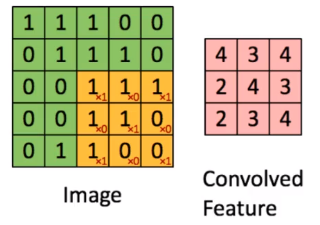
\includegraphics[width=0.75\textwidth]{figures/convolusi.PNG}
	\caption{Ilustasi gambar pada setiap pergeseran filter}
	\label{labelgambar}
\end{figure}
	Convolutional Neural Network (CNN) adalah salah satu jenis neural network yang biasa digunakan pada data image. CNN bisa digunakan untuk mendeteksi dan mengenali object pada sebuah image.
Secara garis besar CNN tidak jauh beda dengan neural network biasanya. CNN terdiri dari neuron yang memiliki weight, bias dan activation function.
Filter pada dasarnya meluncur diatas setiap posisi yang mungkin pada gambar dan pada setiap bagian yang tumpang tindih mendapatkan elemen berlipat ganda untuk pengadaan dan penambahan konvolusi ini merupakan konsep matrix seperti teknik pengukuran jarak ataupun mengukur korelasi sebuah matrix 
Jika filter sangat berkolerasi dengan potongan gambar maka akan menghasilkan jumlah yang sangat besar dan jika filter sangat berbeda dengan potongan gambar maka akan menghasilkan jumlah yang sangat kecil dalam aktualitas yang disebut konvolusi atau disebut sebagai korelasi silang karena konvolusi merupakan sebuah konsep 


\section{cara untuk mendapatkan kode dan data}
Langkahnya sebagai berikut
\begin{figure}[!htp]
	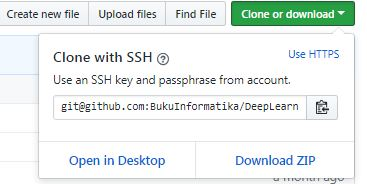
\includegraphics[width=0.75\textwidth]{figures/ssh.JPG}
	\caption{contoh pengambilan kode ssh}
	\label{labelgambar}
\end{figure}

\begin{enumerate}
\item mengambil kode ssh yang ada pada github dan pastikan yang dicopy adalah ssh bukan https
\item jangan lupa melakukan fork terlebih dahulu
\item kemudian disarankan untuk tidak memalsukan repo karena dapat mempersulit 
\end{enumerate}

Dalam hal data, data akan kita temui pada saat kita dalam kuliah dan kursus, beberapa siswa telah meminta saya untuk memberikan 
tentang tutorial latihan coding dalam kursus ini jadi tidak ada alasan lagi untuk tidak dapat mengoding

\begin{enumerate}
\item Dengarkan semua orang dan selamat kembali ke kelas ini jaringan saraf konvolutional canggih dalam kuliah ini saya akan membahas dimana mendapatkan kode untuk kursus ini. Jadi seperti biasa kode dalam kursus ini dapat di unduh dari halaman saya dapatkan, dapatkan progammer dot com slash slash machine contoh pembelajarannya. Untuk mendapatkan kunci tersebut, cobalah untuk mencoba dan menempelkan dari halaman web itu sendiri. Cukup gunakan perintah dapatkan clone lalu buat semua folder yang relevan untuk kursus ini juga kelas CNN.
\item Saya akan mendukung untuk tidak memalsukan repo karena hal ini mempersulit untuk mendapatkan persetujuan dan saya membantah repo cukup banyak terus menerus sehingga anda tidak ingin terjebak dengan versi lama. Selanjutnya jika anda sudah mengambil salah satu kelas saya dan anda sudah memiliki repo ini cukup ketik tarik dan anda secara otomatis memiliki kode untuk data dalam kursus ini.
\item Disetiap bagian dari kursus umumnya akan melihat data set yang berbeda akan menunjukkan dimana untuk mendapatkan data didua tempat, baik dalam kuliah dan dalam kode. Jika anda tidak perlu mengetik apapun yang anda bangkitkan dengan tangan. Perhatikan bahwa dalam kasus dimana kita tidak memerlukan set data besar , tetapi hanya beberapa gambar yang akan dimasukkan dalam laporan itu sendiri. Dalam beberapa kasus , kode nakan sangat baru sehingga anda belum pernah melihatnya sebelumnya.
\end{enumerate}


